\makeatletter\let\ifGm@compatii\relax\makeatother
\documentclass[red]{beamer}

%\usepackage{beamerthemesplit}
\usepackage{listings}
\usepackage{comment}
\usepackage{url}
\usepackage{bm}
\usepackage{tikz}
\usetikzlibrary{arrows.meta}
\usetikzlibrary{shapes.symbols}

\usepackage{hyperref} % has to be last
\hypersetup{
    colorlinks=true,
    linkcolor=blue,
    filecolor=magenta,      
    urlcolor=cyan,
    pdfpagemode=FullScreen,
    }

\tikzset{
    saiarrow/.style={{-Latex}, thick}
}

\newcommand{\isred}[1]{{\color{red} {\bf #1}}} 
\newcommand{\isblue}[1]{{\color{blue}{\bf #1}}} 
\newcommand{\isgreen}[1]{{\color{green} {#1}}} 
\newcommand{\isdarkgreen}[1]{{\color{darkgreen} {#1}}} 
\newcommand{\isorange}[1]{{\color{orange} {#1}}} 

\DeclareMathOperator{\poly}{poly}

\begin{document}


\setbeamercolor{alerted_text}{fg=cyan}
\xdefinecolor{purplish}{cmyk}{0.75,0.75, 0, 0}
\xdefinecolor{purple}{cmyk}{0.75,0.75, 0, 0}
\colorlet{newred}{red!60!black}

\title{Session 7: CPSA formalism, and Beyond CPSA}
\author{Slides prepared by UMBC Protocol Analysis Lab}
\date{Last edited \today}
\begin{frame}
\maketitle
\end{frame}

\begin{frame}\frametitle{How do we know CPSA works?}

\begin{itemize}
\pause
\item CPSA includes a finite set of operations.
\pause
\item Operations provably preserves properties of the protocol.
\pause
\item If CPSA terminates, then all possible executions have been searched
\pause
\item Liskov, M. D., Rowe, P.D., \& Thayer, F.J.\ (2011, October). \href{https://www.mitre.org/sites/default/files/pdf/12_0038.pdf}{Completeness of CPSA}
\pause
\item Proofs \emph{about} theorem provers are extremely complicated
\begin{itemize}
\pause
\item Important if you are interested in proving things \emph{about} CPSA, rather than \emph{with} CPSA.
\end{itemize}
\end{itemize}
\end{frame}

\begin{frame}\frametitle{Enrich by need}
\begin{itemize}
\pause 
\item Rowe, P.D., Guttman, J.D., \& Liskov, M. D.,\ (2011, October). \href{https://dl.acm.org/doi/abs/10.1007/s10207-016-0319-z}{Measuring protocol strength with security goals}
\pause
\item Scenario + Assumptions + Set of actions possible = analysis
\pause
\item ``Enrichment'' refers to finding plausible actions to explain the scenario
\pause
\item Once the scenario is explained, then a skeleton is called \emph{realized}
\end{itemize}
\end{frame}


\title{Post Quantum Cryptography}
\author{What the future of crypto looks like, but when?}
\date{}
\begin{frame}
\maketitle
\end{frame}

\begin{frame}\frametitle{Beyond CPSA}
CPSA let's us model \emph{structural} attacks on protocols.

\pause
Post-quantum attacks are not abstracted from the primitive, so CPSA cannot consider them.
\end{frame}

\begin{frame}\frametitle{Shor's and Grover's algorithms}
\pause
\href{https://ieeexplore.ieee.org/document/365700}{Shor's algorithm} states that an \(n\) bit cryptographic key can be factored in \(\poly(n)\) time.

\pause
Shor's algorithm is \emph{terrifying}, but the largest number factored by a quantum computer is
\pause
21.
\pause
That's right, 21.

\pause
\href{https://dl.acm.org/doi/10.1145/237814.237866}{Grover's algorithm} states that a quantum computer can perform a table lookup in \(O(\sqrt n)\) time, instead of \(O(n)\) time.

\pause
Grover's algorithm permits faster brute-force operations, effectively cutting keysize in half.
An AES-256 key becomes as secure as an AES-128 key.

\pause
Grover's algorithm has, so far, not been shown to be feasible.
\end{frame}

\begin{frame}\frametitle{NIST PQC competition}
\begin{itemize}
\pause
\item National Institute for Standards and Technology (NIST) competition for a new encryption algorithm
\pause
\item Several algorithms submitted, many broken
\pause
\item CRYSTALS-Kyber chosen as the round winner for Key Encapsulation (KEM).
\pause
\item Lattice problem as trapdoor, average case NP-hard
\end{itemize}
\begin{figure}
    \centering
    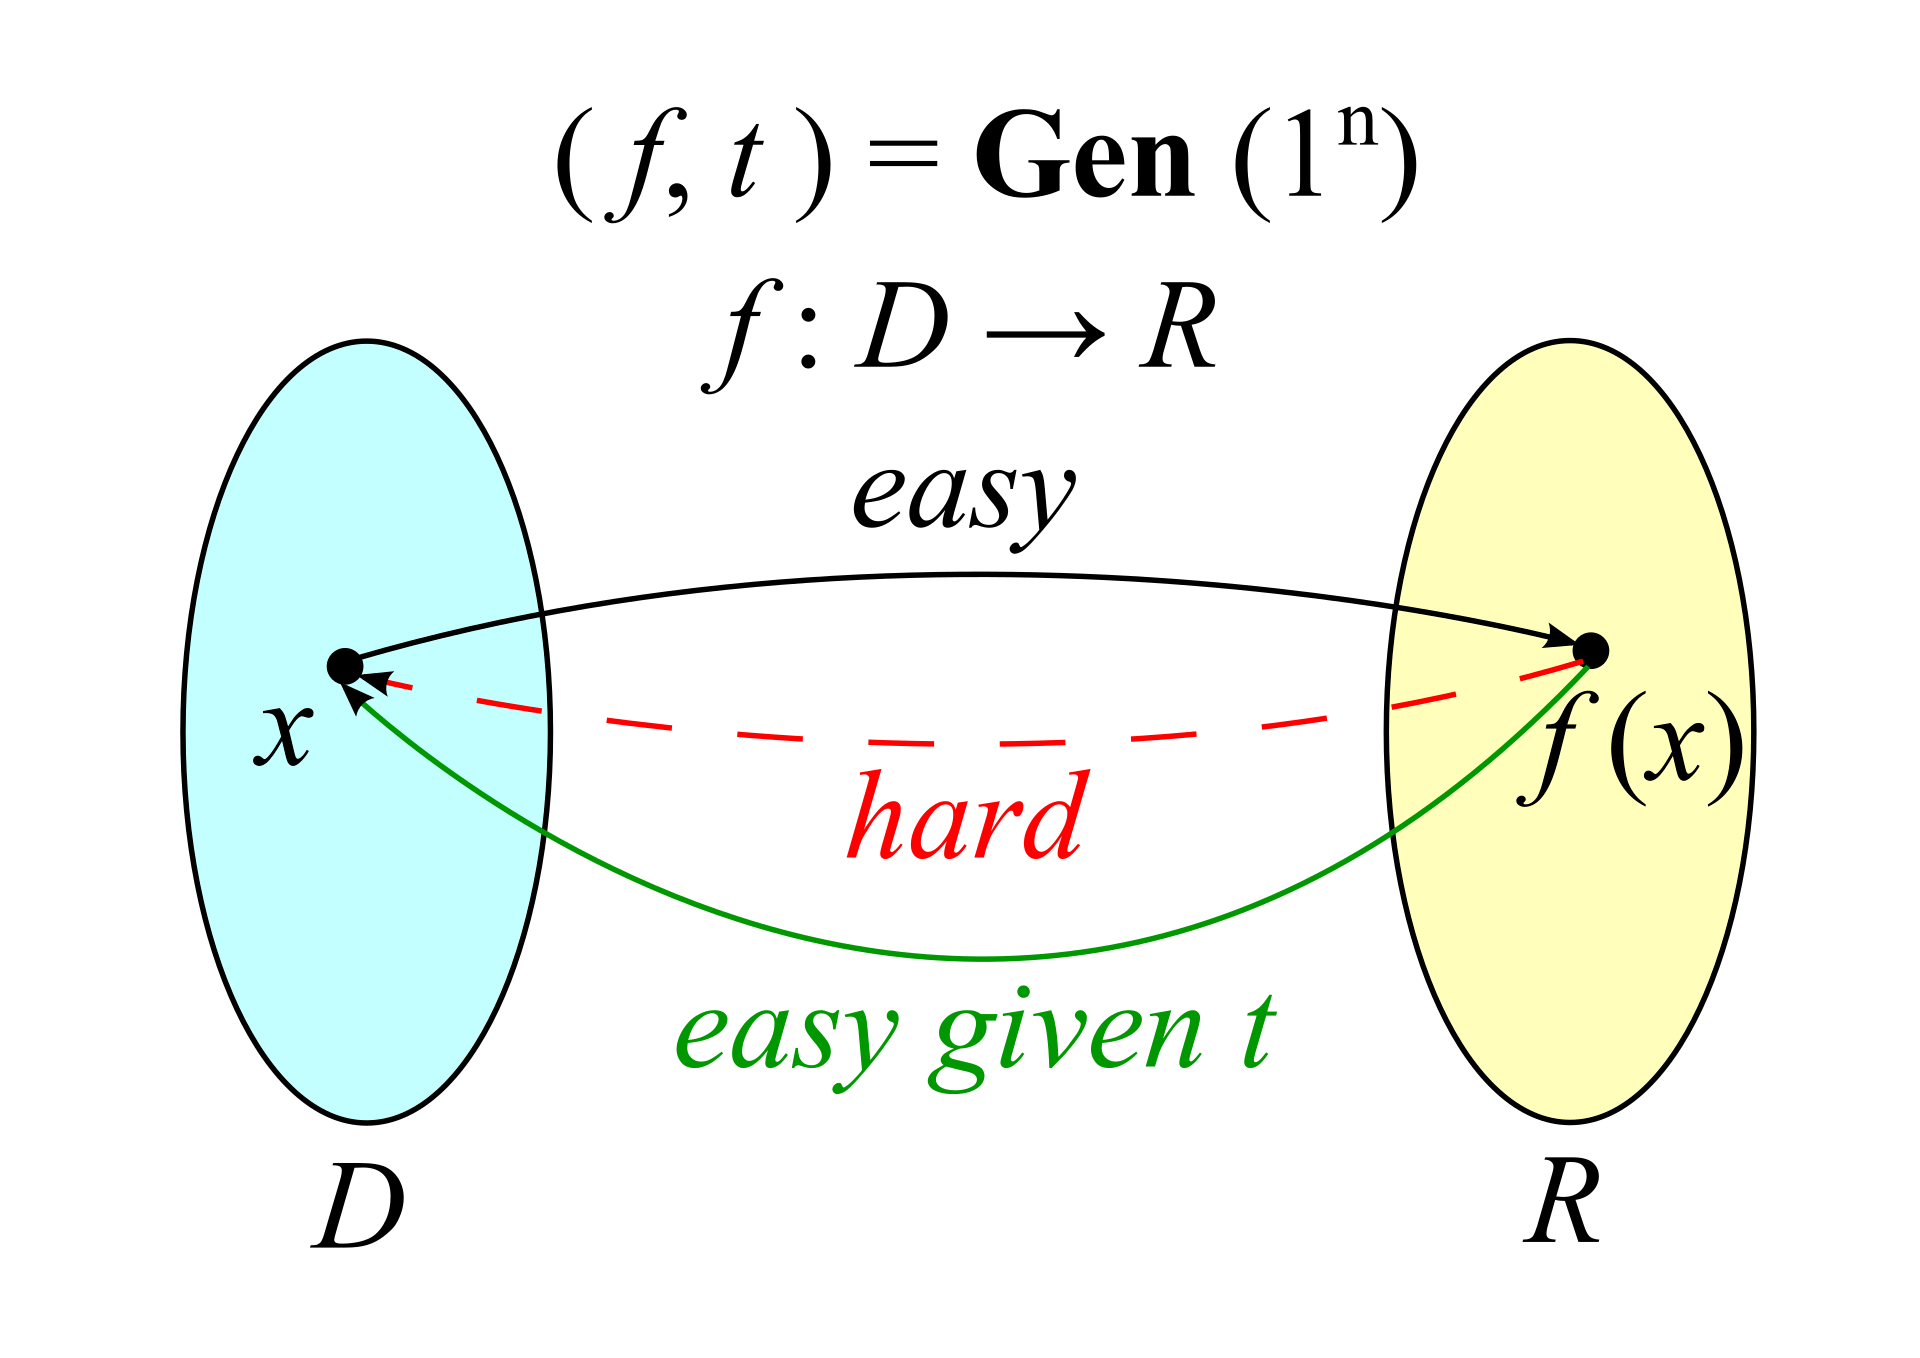
\includegraphics[width=0.55\linewidth]{slide-images/trapdoor.png}
    \caption{\tiny By IkamusumeFan - Own work, CC BY-SA 4.0, https://commons.wikimedia.org/w/index.php?curid=45284265}
\end{figure}

\end{frame}

\begin{frame}\frametitle{Symmetric keys}
\pause
\begin{itemize}
\item Symmetric keys also work for post-quantum security (Large keys because of Grover's)
\pause
\item Biclique attack not feasible on quantum computers
\pause
\item Symmetric key schemes require both parties to have the same key (hard)
\pause
\item Symmetric key schemes can be vulnerable to other attacks
\end{itemize}
\end{frame}

\begin{frame}\frametitle{Merkle signature scheme}
\begin{itemize}
\pause
\item Signature scheme based on hash trees.
\pause
\item Only assumption is the existence of secure hash functions
\pause
\end{itemize}

\begin{figure}
    \centering
    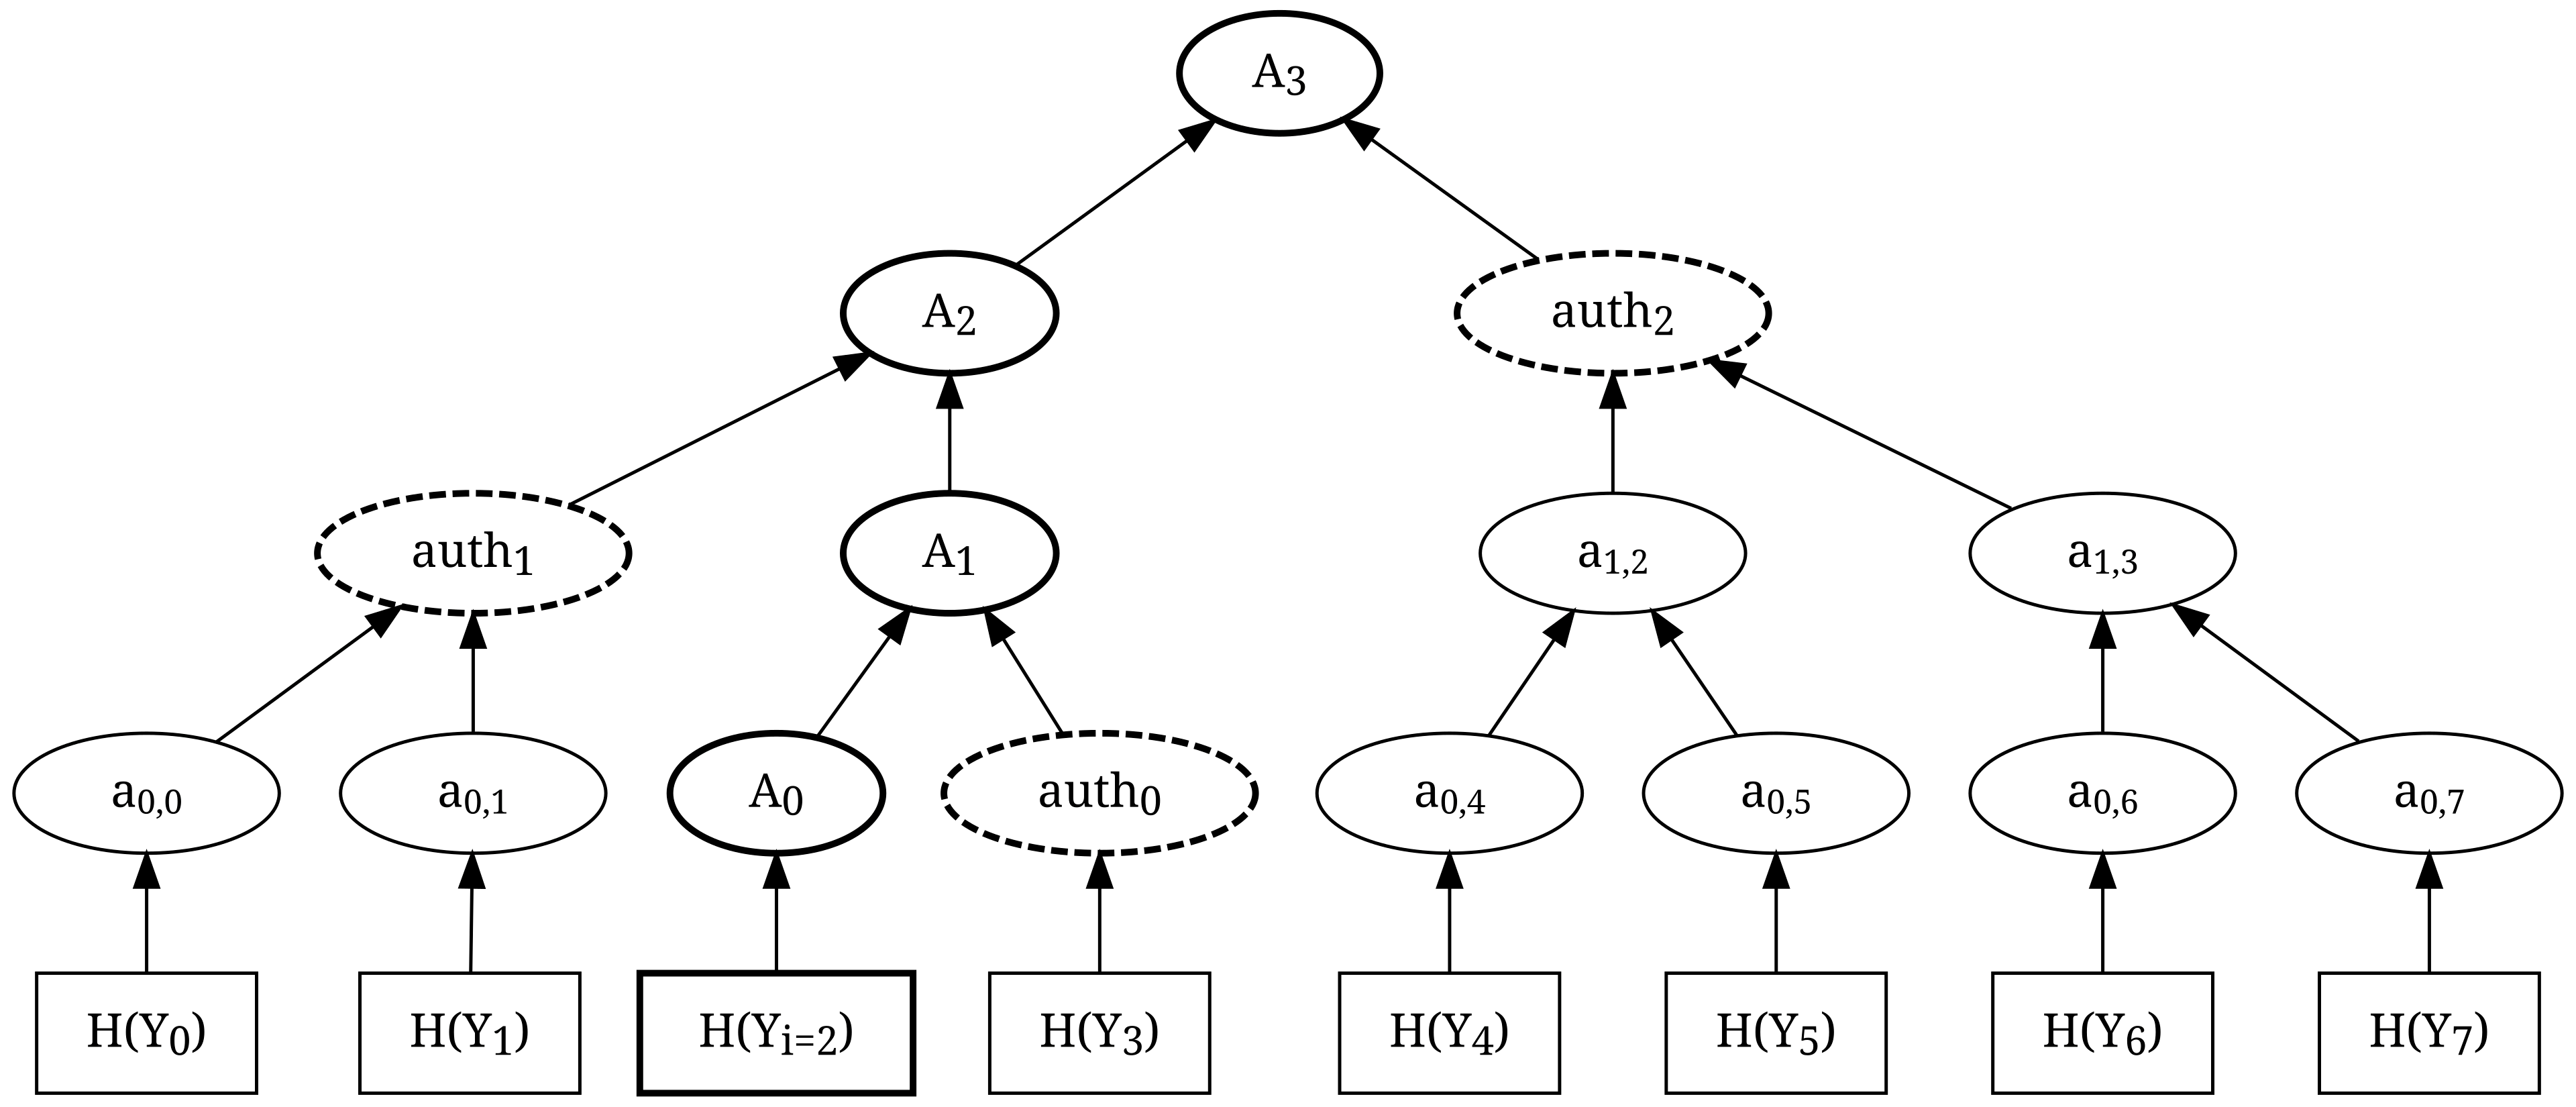
\includegraphics[width=1\linewidth]{slide-images/merkle-signature.png}
    \caption{\tiny By MaxLevy137 - Own work, CC BY-SA 4.0, https://commons.wikimedia.org/w/index.php?curid=69548097}
\end{figure}

\end{frame}

\begin{frame}\frametitle{Survey}
Fill in details about the survey here!
\end{frame}
\end{document}